\documentclass{beamer}
\beamertemplatenavigationsymbolsempty
\usecolortheme{beaver}
\setbeamertemplate{footline}[page number]
\setbeamertemplate{itemize item}{\textendash}
\usepackage{fontspec}
\setmainfont{cmunrm.otf}[BoldFont=cmunbx.otf,ItalicFont=cmunti.otf,BoldItalicFont=cmunbi.otf]
\setsansfont{cmunss.otf}[BoldFont=cmunsx.otf,ItalicFont=cmunsi.otf,BoldItalicFont=cmunso.otf]
\usepackage[english,russian]{babel}
\usepackage{amsmath,amssymb,booktabs,graphicx}
\usepackage{tikz}
\usetikzlibrary{arrows.meta}
\graphicspath{{figures/}}
\title{Microwave circuits wave propagation}
\subtitle{Лабораторная № 2: интервенции и выбор элементов графа}
\author{}\institute{Foundation models for spatial-time series}\date{21 октября 2026}
\begin{document}
\begin{frame}\maketitle\vspace{-1em}\begin{center}\small
Основа: первая лабораторная gkarpeev/maxwell.\\
Синтетика и экспериментальные измерения СВЧ-линии.
\end{center}\end{frame}

\begin{frame}{От Максвелла к наблюдаемой волне}\small
В нормировке первой лабораторной, $\mu_r=1$:
\[
\partial_t\mathbf e=\frac{c}{\epsilon_r}\nabla\times\mathbf h
-\frac{\sigma}{\epsilon_0\epsilon_r}\mathbf e,\quad
\partial_t\mathbf h=-c\nabla\times\mathbf e.
\]
Для одной гармонической TEM-моды:
\[
E_y(x,t)=\Re\{E_0e^{-\gamma x}e^{i\omega t}\},\qquad\gamma=\alpha+i\beta.
\]
Эффективная модель малых потерь, $u=f/(10\,\text{ГГц})$:
\[
\alpha=a\sqrt u+b u,\qquad \beta=\frac{2\pi f}{c}n+a\sqrt u.
\]
\begin{itemize}
\item $n$ --- показатель преломления; $a$ --- проводниковый вклад.
\item $b$ --- дополнительный частотный член потерь; $a,b$ в Нп/м.
\item Это гармоническая редукция PDE; частоты не являются кадрами времени.
\end{itemize}
\end{frame}

\begin{frame}{Что переиспользовано и какие данные добавлены}\small
\begin{itemize}
\item Из работы \href{https://github.com/gkarpeev/maxwell}{gkarpeev/maxwell}: типизированный DAG,
уравнения, аналитические волны, FDTD-проверка и подбор параметра. Исходники сохранены без изменений.
\item Проверка: найдено $\epsilon_r\approx4$ при эталоне 4;
при уточнении сетки $12^3\to24^3$ ошибка уменьшается в $3.913$ раза.
\item Наборы PDEArena и EMVal у автора синтетические.
\item Для реальной части добавлены измерения Hatab et al.:
воздушная коаксиальная линия, 10 положений подвижного элемента, три VNA.
\end{itemize}
Основной набор: ZNA, 151 частота, 3--18 ГГц.
Обучение: 119 частот; контроль: 32 в отдельных полосах.
\medskip

\scriptsize\href{https://doi.org/10.3390/s23094548}{Hatab et al., Sensors 23, 4548 (2023)};
\href{https://doi.org/10.3217/6bd26-5cp67}{данные и авторский алгоритм}.
Измерены S-параметры, из них извлечена $\gamma$; объёмные поля $E,H$ не измерялись.
\end{frame}

\begin{frame}{Тройка методов}\small
\begin{enumerate}
\item \textbf{Блочный бутстреп:} 1000 реплик, блок 8 соседних частот;
сохраняются пары $(\alpha,\beta)$. Проверка блоков 4 и 12.
\item \textbf{Условное зашумление:}
\[
y_j^{(\lambda)}(f)=y_j(f)+\lambda s_j(f)z_j^*,\quad
\lambda\in\{0,0.5,1,2,4\}.
\]
Масштаб и парные блочные остатки оцениваются только по обучению.
Шум в $\alpha$, в $\beta$ либо в оба канала.
\item \textbf{Wasserstein-1:} эмпирические распределения без оценки плотности.
Нормировка на исходное SD; совместно --- 128 проекций sliced-W1.
\end{enumerate}
\medskip
Сравниваются квадратичная ошибка и soft-L1.
Это вычислительное вмешательство в данные, а не физическое изменение установки.
\end{frame}

\begin{frame}{Параметры и элементы графа}
\centering
\begin{tikzpicture}[x=1cm,y=.95cm,every node/.style={draw,rounded corners,minimum width=1.1cm,minimum height=.45cm,font=\small},every edge/.style={draw,-{Stealth}}]
\node[fill=blue!10] (u) at (-4.7,0) {$f/f_0$};
\node[fill=orange!25] (b) at (-3.1,0) {$b$};
\node[fill=blue!10] (s) at (-.8,0) {$\sqrt{f/f_0}$};
\node[fill=orange!25] (a) at (.8,0) {$a$};
\node[fill=blue!10] (k) at (3.1,0) {$\omega/c$};
\node[fill=orange!25] (n) at (4.7,0) {$n$};
\node[fill=green!10] (m1) at (-3.9,-1) {$\times$};
\node[fill=green!10] (m2) at (0,-1) {$\times$};
\node[fill=green!10] (m3) at (3.9,-1) {$\times$};
\node[fill=green!10] (alpha) at (-2,-2) {$\alpha:\;+$};
\node[fill=green!10] (beta) at (2,-2) {$\beta:\;+$};
\path (u) edge (m1) (b) edge (m1) (s) edge (m2) (a) edge (m2)
(k) edge (m3) (n) edge (m3) (m1) edge (alpha) (m2) edge (alpha)
(m2) edge (beta) (m3) edge (beta);
\end{tikzpicture}
\small
\begin{itemize}
\item $n$: фазовый вклад; проверяется замена на $n=1$, не на ноль.
\item $a$: общий узел и оба пути в затухание и фазу.
\item $b$: ветвь $b(f/f_0)$ и вход в сумму затухания.
\end{itemize}
\footnotesize Матрица и порядок аргументов сохранены. Удаление $b$ не удаляет все потери или уравнение Максвелла.
\end{frame}

\begin{frame}{Измерения и подобранная модель}
\centering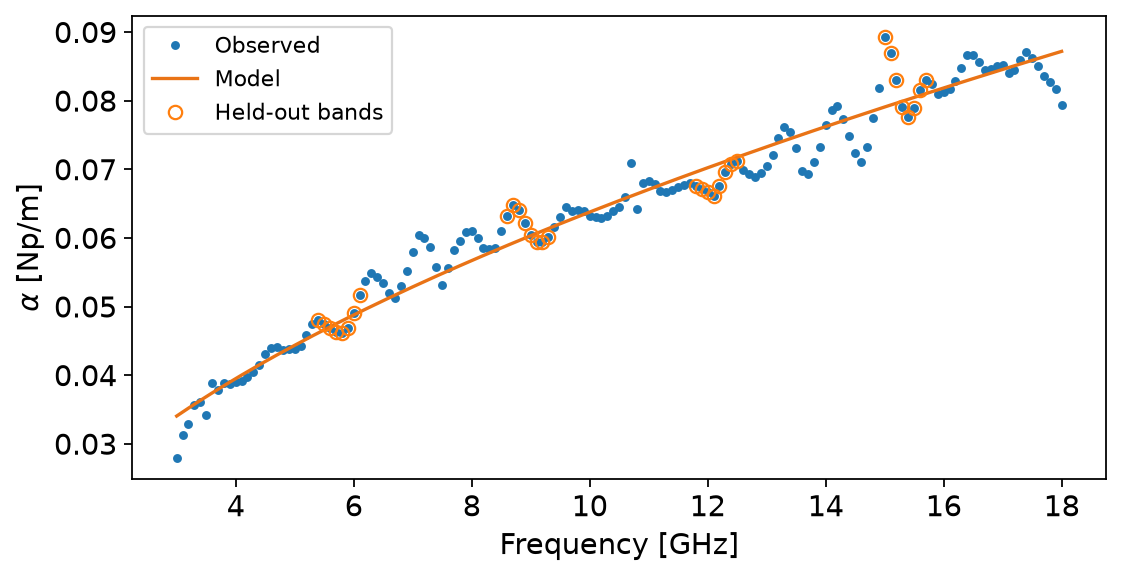
\includegraphics[width=.87\textwidth]{slide_fit.png}
\small
\[
n=1.0033176,\qquad a=0.06019\ \text{Нп/м},\qquad b=0.00357\ \text{Нп/м}.
\]
RMSE на контроле: $\alpha$ --- $0.00327$ Нп/м;
$\beta$ --- $0.00945$ рад/м.
\medskip

\footnotesize Фазовый канал заметно крупнее по масштабу, поэтому ошибки двух каналов нормируются отдельно.
\end{frame}

\begin{frame}{Как изменяются распределения параметров}
\centering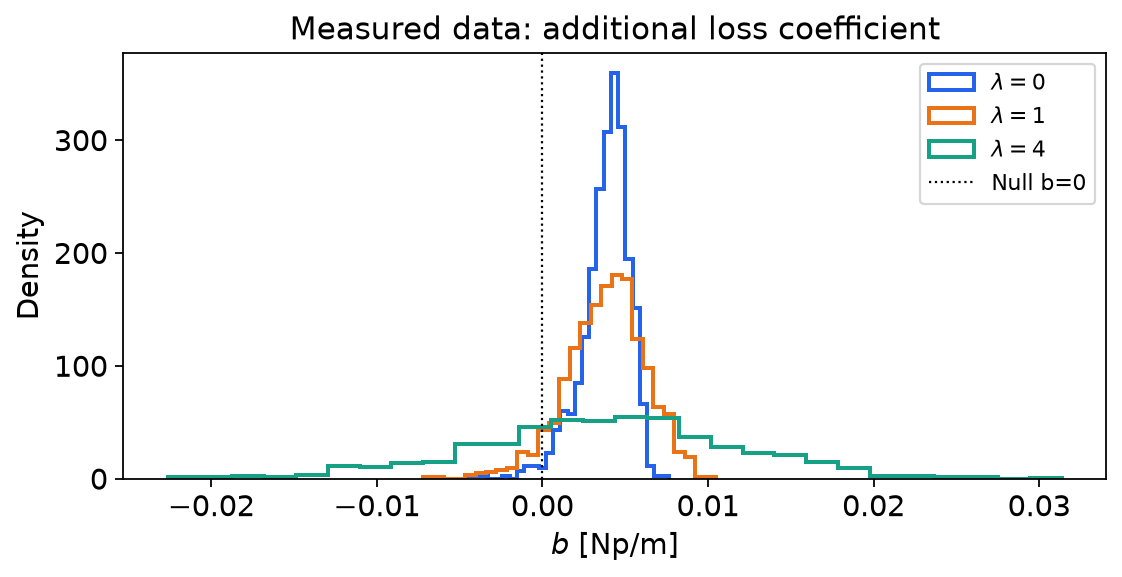
\includegraphics[width=.87\textwidth]{slide_distribution.png}
\small
При усилении шума меняются разброс и положение оценок.
Это не означает изменения истинной среды.
\medskip

\footnotesize В ноутбуке показаны оба набора, обе функции ошибки,
совместные распределения и отдельные вмешательства в $\alpha,\beta$.
\end{frame}

\begin{frame}{Расстояние от силы вмешательства}
\centering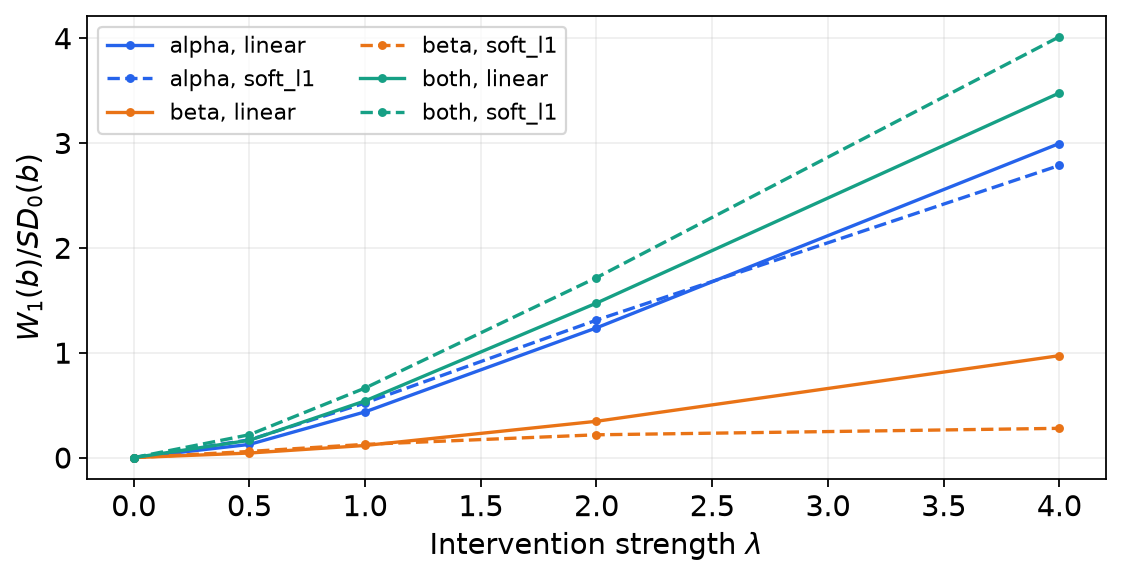
\includegraphics[width=.87\textwidth]{slide_distance.png}
\small
Нормировочное SD фиксировано по исходному бутстрепу.
При $\lambda=0$ расстояния точно равны нулю.
\medskip

\footnotesize Большое расстояние показывает чувствительность оценки,
но само по себе не разрешает удалить ветвь. Для связанных $a,b$ также проверяется sliced-W1.
\end{frame}

\begin{frame}{Критерий и решение}\small
Удаление допустимо, только если:
\begin{enumerate}
\item 95\%-й интервал содержит нулевой вклад;
\item после повторного подбора остальных параметров верхняя граница прироста
контрольного RMS $\le0.25$ единицы остаточного шума;
\item при $\lambda=1$ выполнено $W_1/SD_0\le1$;
\item решение подтверждается при блоках 4, 8 и 12.
\end{enumerate}
\centering
\begin{tabular}{lcc}\toprule
Вклад & Синтетика & Измерения\\\midrule
$n$ & Сохранить & Сохранить\\
$a$ & Сохранить & Сохранить\\
$b$ & Удалить & Сохранить\\\bottomrule
\end{tabular}
\medskip

\footnotesize В генераторе синтетики $b=0$.
На измерениях вывод о $b$ меняется с длиной блока: устойчивое удаление не подтверждено.
Допуски --- учебный выбор, не универсальный статистический тест.
\end{frame}

\begin{frame}{Ограничения и источники}\footnotesize
\begin{itemize}
\item Вывод относится к эффективной модели и полосе 3--18 ГГц.
Остатки могут включать ошибку модели; полной неопределённости VNA здесь нет.
\item Контроль участвует в выборе структуры. Это не окончательный независимый тест.
\end{itemize}
\medskip
\begin{enumerate}
\item \href{https://github.com/gkarpeev/maxwell}{gkarpeev/maxwell}, первая лабораторная; commit b88901c.
\item Oskooi et al., Meep (2010): \href{https://doi.org/10.1016/j.cpc.2009.11.008}{doi:10.1016/j.cpc.2009.11.008}.
\item Hatab et al. (2023): \href{https://doi.org/10.3390/s23094548}{doi:10.3390/s23094548};
данные \href{https://doi.org/10.3217/6bd26-5cp67}{doi:10.3217/6bd26-5cp67}.
\item Bobowski (2020): \href{https://arxiv.org/abs/2006.14381}{arXiv:2006.14381}.
\item Efron (1979): \href{https://doi.org/10.1214/aos/1176344552}{doi:10.1214/aos/1176344552}.
Künsch (1989): \href{https://doi.org/10.1214/aos/1176347265}{doi:10.1214/aos/1176347265}.
\item \href{https://docs.scipy.org/doc/scipy/reference/generated/scipy.stats.wasserstein_distance.html}{SciPy: Wasserstein-1};
\href{https://docs.scipy.org/doc/scipy/reference/generated/scipy.optimize.least_squares.html}{TRF и soft-L1}.
\end{enumerate}
\end{frame}
\end{document}
